\chapter{مفاهیم پایه}

در این فصل به معرفی تکنولوژی و فریمورک های به کار رفته در پروژه میپردازیم.

\section{Firecracker}
در قلب پروژه Firecracker قرار دارد. Firecracker یک مانیتور ماشین مجازی است که از KVM استفاده می‌کند و
وظیفه اش ساخت و مدیریت ماشین های مجازی است.
Firecracker توسط تیم وب سرویس آمازون توسعه داده شده و در پروژه Fargate و Lambda این شرکت نیز استفاده شده است.

\begin{figure}[h]
    \centering
    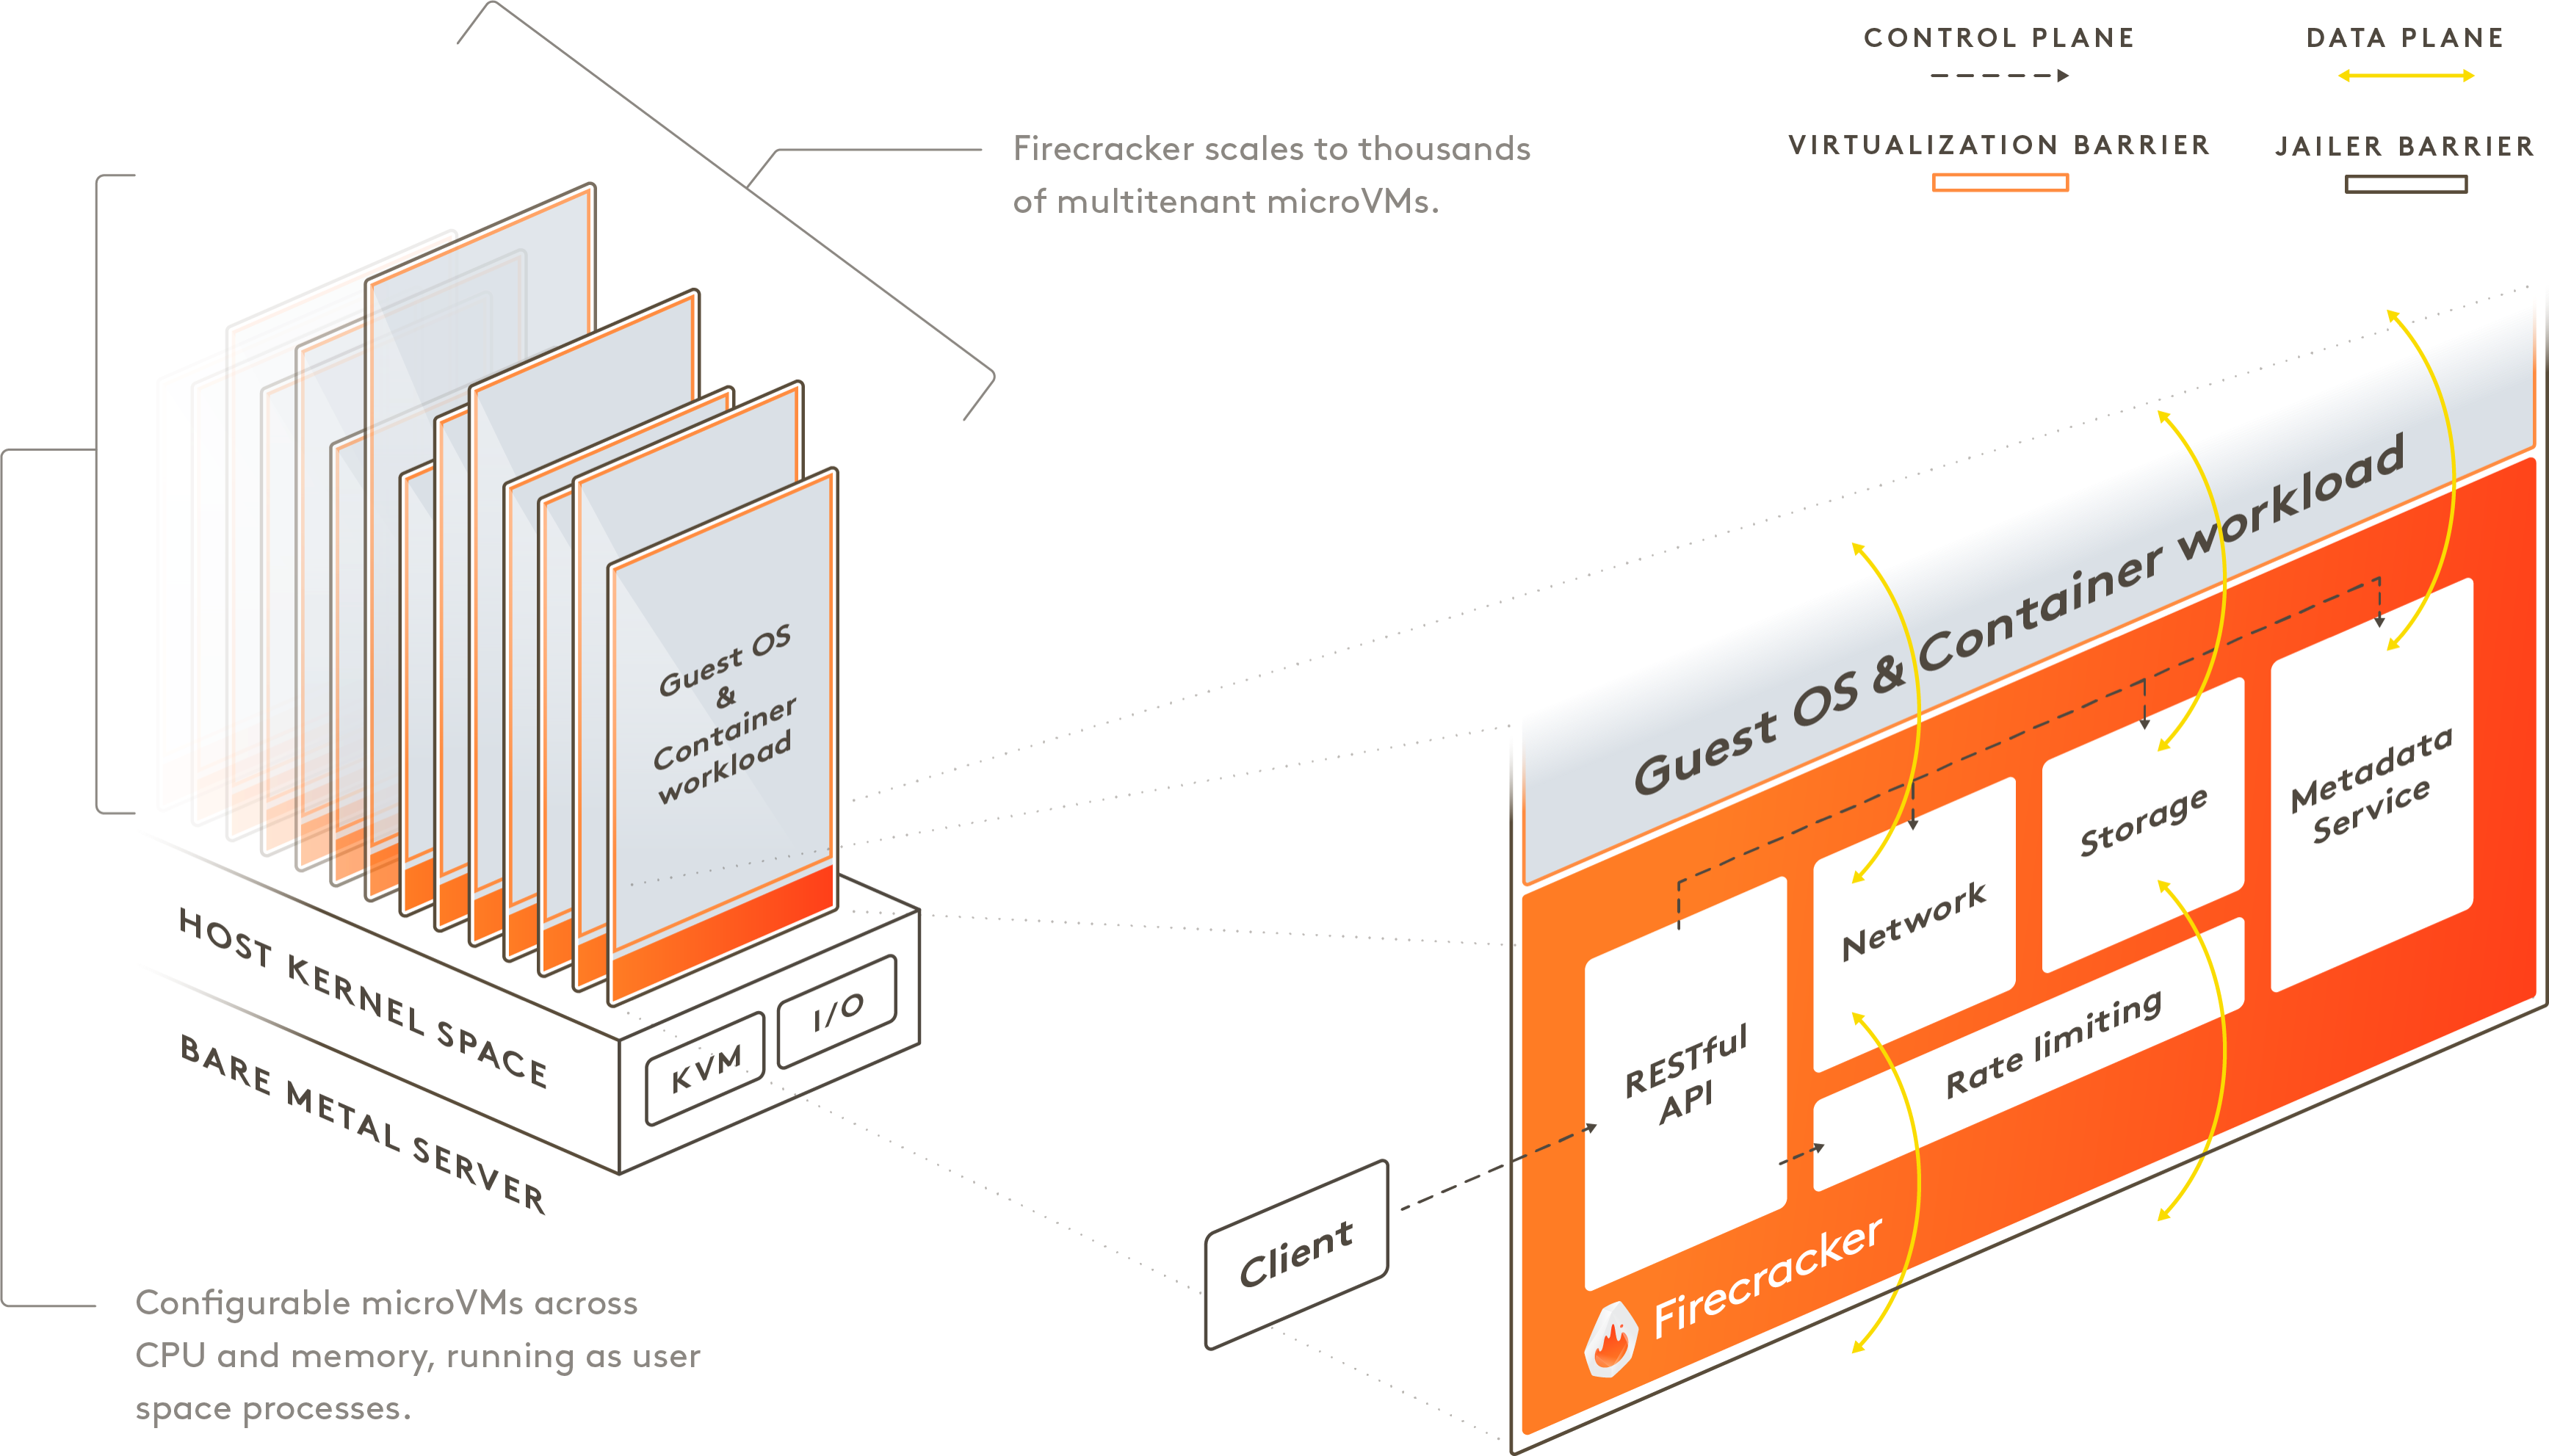
\includegraphics[width=0.7\textwidth]{./1-Introduction/firecracker-diagram.png}
    \caption{a nice plot}
    \label{fig:mesh1}
\end{figure}

\section{Go Fiber}
زبان استفاده شده در میکروسرویس ها Go می‌باشد و از فریمورک Fiber استفاده شده که برای ساده تر شدن routing و middleware استفاده شده است.

\section{RabbitMQ}

\section{PostgreSQL}

\section{Next.js}
فریمورک استفاده شده سمت کلاینت Next.js می‌باشد که از کتابخانه React برای رندر روی مرورگر استفاده میکند.


زبان برنامه نویسی سمت کلاینت TypeScript است که به واسطه کامپایلر تبدیل به JavaScript می‌شود.
دلیل استفاده از TypeScript اضافه شدن شی‌گرایی و تایپ در زمان کامپایل است.
